\chapter{基于神经网络预测太阳黑子变化}\label{chap:ml_sunspot}

要进行机器学习,先要有数据集。数据集由很多样本组成。在研究太阳黑子变化时,只考虑了历史太阳黑子变化如何影响未来太阳黑子变化。因此模型的输入和输出都来自同一种特征。本论文从一种特征(太阳黑子强度)出发,利用机器学习探索时间序列数据。

\section{研究背景}\label{sec:ss_intro}

太阳活动是太阳大气中局部区域各种不同活动现象的总称,包括太阳黑子、日珥、光斑、谱斑、耀斑、太阳风和日冕质量抛射等。处于活动剧烈期的太阳会辐射出大量紫外线、X射线、粒子流和强射电波,导致地球上出现极光、磁暴和电离层扰动等现象。太阳活动对地球的影响有以下几个方面\citep{jie2012prediction}:
\begin{itemize}
  \item[$\circ$] \textbf{地球大气层}。地球大气层在太阳的辐射下形成电离层,无线电波依靠电离层的反射向远距离传播。当太阳活动剧烈时,在向阳的半球电离层容易衰减甚至中断。
  \item[$\circ$] \textbf{地球气候}。太阳活动周期与地球气候的关系也比较明显,其作用机制并不清楚。太阳活动达到高峰时,地球上太平洋热带及亚热带地区气温升高、海水加速蒸发、西太平洋热带海域的降雨增多,东太平洋热带海域气温降低。
  \item[$\circ$] \textbf{地球磁场}。太阳活动剧烈时,地球磁场会产生磁暴现象。
  \item[$\circ$] \textbf{航天活动}。大耀斑出现时,会射出的高能量质子,对航天飞行、卫星设备、太阳能电池等有极大的破坏性。
\end{itemize}

太阳黑子是太阳局部强磁场活动在太阳光球层上产生的黑色斑块,是太阳活动强弱的很容易观测到的特征。\citet{noyes2013sun}详细阐述了太阳黑子的产生机制。太阳黑子位于太阳表面的强磁场区,是太阳表面的炽热气体形成的巨大漩涡,温度高达3000$^{\circ}$C-4500$^{\circ}$C。太阳黑子由太阳大气中的电磁过程引起,时烈时弱,平均以$\sim$11年为周期。通常太阳黑子数量越多,太阳活动越频繁。太阳黑子可以成群出现,也可以是单个孤立的本影,周围有半影。

传统意义上,基于半经验性的物理机制模型和基于统计学模型已经被广泛应用于太阳黑子时间序列预测。然而,这些模型都有一个前提假设,时间序列是从线性过程产生的,难以有效地抓住非高斯型、非稳态型和非线性的时间序列关系\citep{jiang2011sunspot,arlt2015solar}。

近些年来,机器学习中的神经网络在太阳黑子预测中的应用非常普遍\citep{pala2019forecasting}。使用的神经网络模型愈加复杂,容错能力也逐渐增加。例如,\citet{zhao2008prediction}使用径向基神经网络预测未来4个月的平滑月均太阳黑子数,发现相对误差控制在38\%以内,而且误差会随着预测时间的延长而逐渐增加;\citet{ding2012prediction}基于反向传播神经网络(Backpropagation Neural Network,简称BPNN)预测平滑月均太阳黑子面积,发现相对误差不超过5\%;\citet{li2018hybrid}在预测太阳黑子数时,使用了BPNN及其变种的神经网络,发现组合的神经网络强于BPNN,RMSE为1.7117,MAPE为0.0435。

尽管很多学者基于年/月均太阳黑子时间序列数据利用不同的模型预测未来一个太阳周(尤其是第25太阳周)的峰值,却没有得出一个统一的结论。对于第23太阳周而言,峰值出现时间为2001年9月,此时太阳黑子数为238.2,太阳黑子面积为2171.7;对于第23太阳周而言,峰值出现时间为2014年2月,此时太阳黑子数为146.1,太阳黑子面积为1439.8。对于预测的第25太阳周太阳黑子强度,可分为以下几种结论:
\begin{enumerate}
  \item[(1)] 与第24太阳周相比,第25太阳周太阳黑子更强。也就是说,太阳黑子可能不会大幅减弱,甚至可能扭转太阳活动大幅减弱的趋势。例如,\citet{mcintosh2020overlapping}基于磁活动周期的物理模型,预测到第25太阳周是有史以来观察到的最强的太阳黑子周期之一,峰值为$\sim$233;\citet{pesnell2018effects}采用na{\"\i}ve方法,得到第25太阳周的太阳黑子数为$\sim$180\pm 60。
  \item[(2)] 与第24太阳周相比,第25太阳周太阳黑子强度基本与之持平。例如,\citet{hiremath2008prediction}预测未来$\sim$170年的太阳黑子变化,发现第24和25太阳周的太阳黑子数均为$\sim$110;\citet{bhowmik2018prediction}得到第25太阳周的太阳黑子数为$\sim$118,出现在$\sim$2024年;\citet{singh2019prediction}得出第25太阳周太阳黑子数峰值为124\pm 11,出现在2024年2月;\citet{bisoi2020another}得出第25太阳周太阳黑子数峰值为$\sim$131--134,出现在2025年7月。
  \item[(3)] 与第24太阳周相比,第25太阳周太阳黑子更弱。例如,\citet{kitiashvili2020application}发现第25太阳周的最大太阳黑子数为$\sim$50(发生在2024年或2025年)。该数值小于Dalton最低点期间的太阳黑子数,可能与Maunder最低点相当。
\end{enumerate}

总之,无论最终模型的表现效果如何,目前很难对未来第25太阳周太阳黑子活动的非线性动态特征(太阳黑子峰值和太阳周持续时间)进行精准预测。究其原因,太阳黑子时间序列具有非平稳型、非高斯型、非线性特征。目前,有关太阳黑子的记录长达400多年,太阳黑子时间序列数据显示出周期性震荡。通过机器学习探索太阳黑子变化的趋势,有助于理解太阳活动的机制。鉴于预测未来第25太阳周太阳黑子活动难以取得一致性的结果,本章尝试预测未来1个月和72个月的太阳黑子变化,将未来72个月的最大太阳黑子强度定义为第25太阳周的峰值,探索在什么情况下能够较为精准地预测太阳黑子强度。

本章结构安排如下。第\ref{sec:ss_data_method}节描述了太阳黑子时间序列和预处理过程。第\ref{sec:ss_result}节描述太阳黑子变化的试验过程,并将试验结果可视化。第\ref{sec:ss_conclusion}节对预测太阳黑子动态变化进行了总结与展望。

\section{数据与方法}\label{sec:ss_data_method}

本节首先介绍了太阳黑子数量和面积的时间序列以及两者长期的变化趋势。接着介绍原始数据集进行预处理的过程,包括生成监督学习数据集、数据集划分、归一化处理等。最后选取几种不同结构的神经网络训练处理后的数据。

\subsection{数据简介}\label{sec:ss_dataset}

\begin{table}[!htbp]
  \centering
  \bicaption[13个月平滑的月均太阳黑子数量、峰值和谷值出现的时间]{13个月平滑的月均太阳黑子数量、峰值和谷值出现的时间。}{Solar minimum and maximum timings and amplitudes of 13-month smoothed monthly mean sunspot numbers.}
  \label{tab:ss_max_min}
  \footnotesize
  \begin{tabular}{cccccccc}
    \toprule
    \multicolumn{1}{c}{}&\multicolumn{2}{c}{谷值}&
    \multicolumn{2}{c}{峰值}& \multicolumn{3}{c}{时间(年)}\\
    \cmidrule(lr){2-3} \cmidrule(lr){4-5} \cmidrule(lr){6-8} \noalign{\smallskip}
    \multicolumn{1}{c}{太阳周} & 日期 & 黑子数 & 日期 & 黑子数 & 上升 & 下降 & 最小值到最小值\\ 
    \midrule 
    1 & 1755.204 & 14.0 & 1761.455 & 144.1 & 6.251 & 5.000 & 11.251 \\
    2 & 1766.455 & 18.6 & 1769.707 & 193.0 & 3.252 & 5.748 & 9.000 \\
    3 & 1775.455 & 12.0 & 1778.371 & 264.3 & 2.916 & 6.337 & 9.253 \\
    4 & 1784.708 & 15.9 & 1788.124 & 235.3 & 3.416 & 10.164 & 13.580 \\
    5 & 1798.288 & 5.3 & 1805.123 & 82.0 & 6.835 & 5.835 & 12.670 \\
    6 & 1810.958 & 0.0 & 1816.373 & 81.2 & 5.415 & 6.998 & 12.413 \\
    7 & 1823.371 & 0.2 & 1829.874 & 119.2 & 6.503 & 4.000 & 10.503 \\
    8 & 1833.874 & 12.2 & 1837.204 & 244.9 & 3.330 & 6.334 & 9.664 \\
    9 & 1843.538 & 17.6 & 1848.124 & 219.9 & 4.586 & 7.834 & 12.420 \\
    10 & 1855.958 & 6.0 & 1860.124 & 186.2 & 4.166 & 7.080 & 11.246 \\
    11 & 1867.204 & 9.9 & 1870.623 & 234.0 & 3.419 & 8.335 & 11.754 \\
    12 & 1878.958 & 3.7 & 1883.958 & 124.4 & 5.000 & 6.246 & 11.246 \\
    13 & 1890.204 & 8.3 & 1894.042 & 146.5 & 3.838 & 8.000 & 11.838 \\
    14 & 1902.042 & 4.5 & 1906.123 & 107.1 & 4.081 & 7.500 & 11.581 \\
    15 & 1913.623 & 2.5 & 1917.623 & 175.7 & 4.000 & 6.000 & 10.000 \\
    16 & 1923.623 & 9.4 & 1928.290 & 130.2 & 4.667 & 5.417 & 10.084 \\
    17 & 1933.707 & 5.8 & 1937.288 & 198.6 & 3.581 & 6.836 & 10.417 \\
    18 & 1944.124 & 12.9 & 1947.371 & 218.7 & 3.247 & 6.917 & 10.164 \\
    19 & 1954.288 & 5.1 & 1958.204 & 285.0 & 3.916 & 6.587 & 10.503 \\
    20 & 1964.791 & 14.3 & 1968.874 & 156.6 & 4.083 & 7.332 & 11.415 \\
    21 & 1976.206 & 17.8 & 1979.958 & 232.9 & 3.752 & 6.749 & 10.501 \\
    22 & 1986.707 & 13.5 & 1989.874 & 212.5 & 3.167 & 6.750 & 9.917 \\
    23 & 1996.624 & 11.2 & 2001.874 & 180.3 & 5.250 & 7.084 & 12.334  \\
    24 & 2008.958 & 2.2 & 2014.288 & 116.4 & 5.330 & — & —  \\
    平均值 & 9.29 &  & 178.7 & 4.33 & 6.74 & 11.03  \\
    标准差 & 5.70 &  & 57.76 & 1.11 & 1.24 & 1.18 \\
    中值 & 9.65 &  & 183.3 & 4.08 & 6.75 & 11.25 \\
    \bottomrule
  \end{tabular}
\end{table}

\begin{figure}[!htbp]
  \centering
  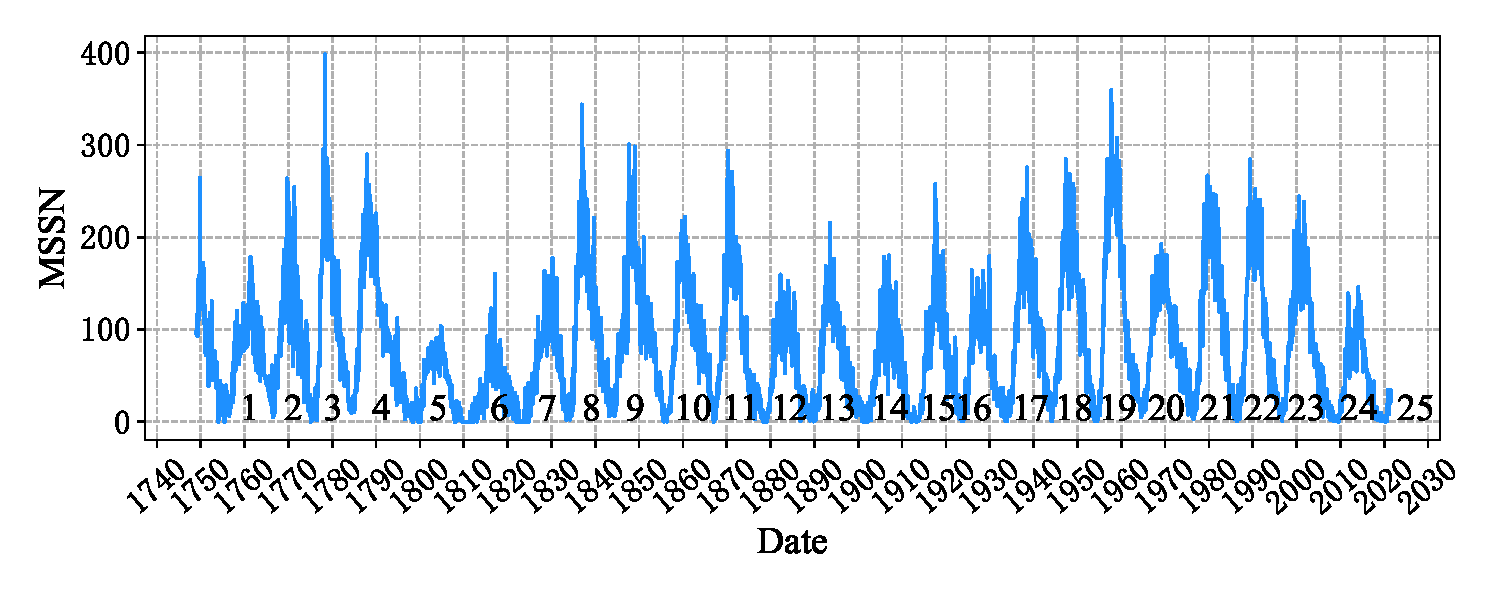
\includegraphics[width=\textwidth]{Img/chap3_ss/ss_number_series.pdf}
  \vspace{-1.4cm}
  \bicaption[1949年至2021年期间月均太阳黑子数]{1949年至2021年期间月均太阳黑子数。}{Monthly mean total sunspot number between 1749 and 2021.}
  \label{fig:ss_number_series}
\end{figure}

本章采用两种时间序列数据集。第一类为月均太阳黑子数(Monthly Mean Total Sunspot Number,简称MSSN),来自SILSO(Sunspot Index and Long-Term Solar Observation)网站\footnote{数据来源:WDC-SILSO,Royal Observatory of Belgium,Brussels,\href{http://sidc.be/silso/datafiles}{http://sidc.be/silso/datafiles}}发布的太阳黑子2.0版本。MSSN数据集跨越了$\sim$273年(从1749年1月至2021年8月),包含3272条记录。截至目前,MSSN数据集包含了24个太阳周。表\ref{tab:ss_max_min}展示了这24个太阳周太阳黑子数量、峰值和谷值出现时间。第1太阳周为1755年2月至1766年5月,目前正处于第25太阳周的起始阶段\footnote{参考:\href{www://sidc.be/silso/cyclesmm}{www://sidc.be/silso/cyclesmm}}。图\ref{fig:ss_number_series}使用1749年1月至2021年8月期间月均太阳黑子数时间序列数据,绘制了太阳黑子数的变化趋势。图\ref{fig:ss_number_series}显示,MSSN数据集的分布是右偏的。\citet{panigrahi2021forecasting}指出,MSSN数据集的峰度大于3。鉴于MSSN数据集呈现出复杂的非高斯型分布,因此较难预测出太阳黑子数的变化趋势。

\begin{figure}[!htbp]
  \vspace{-0.3cm}
  \centering
  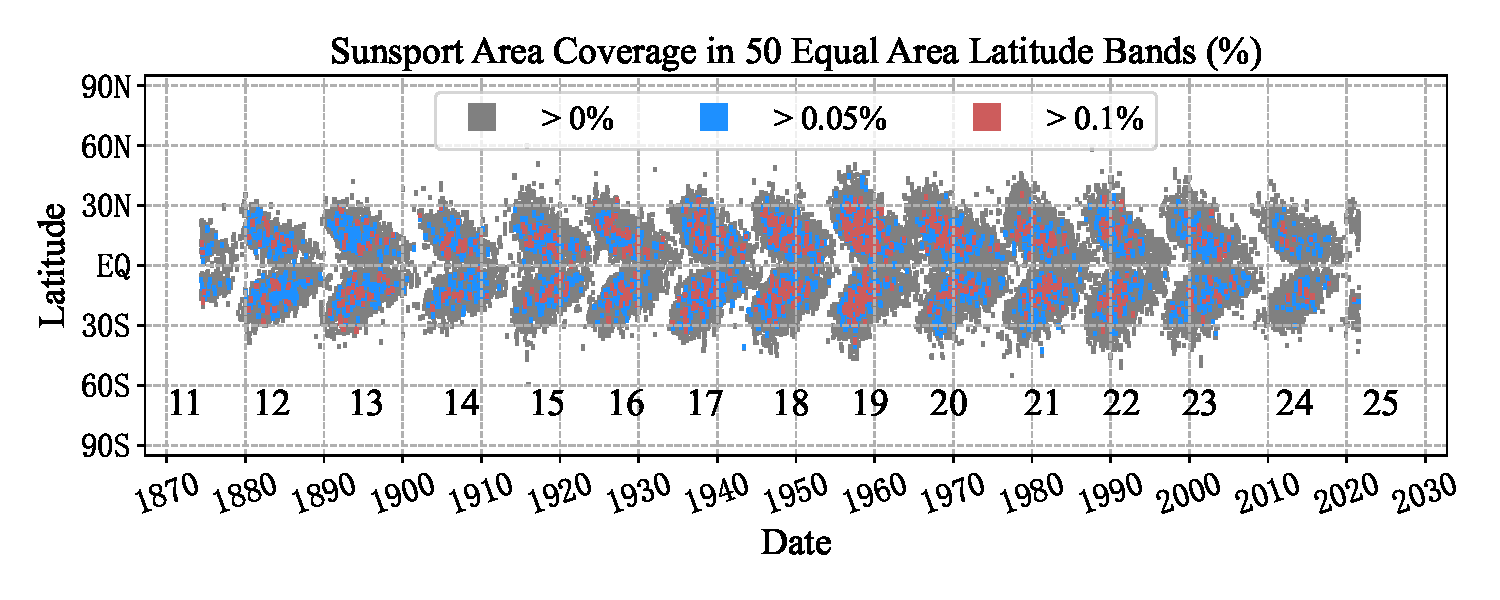
\includegraphics[width=\textwidth]{Img/chap3_ss/ss_butterfly.pdf}
  \vspace{-1.4cm}
  \bicaption[1949年至2021年期间太阳黑子面积随时间和纬度变化的蝴蝶图]{1949年至2021年期间太阳黑子面积随时间和纬度变化的蝴蝶图。}{Butterfly diagram of sunspot area which marks the latitude of sunspot locations as a function of time from 1749 to 2021.}
  \label{fig:ss_butterfly}
\end{figure}

第二类数据集为太阳黑子面积(Sunspot Area,简称SSA)。SSA数据集来自Lisa Upton和David Hathaway提供的网站\footnote{参考:\href{http://solarcyclescience.com/activeregions.html}{http://solarcyclescience.com/activeregions.html}},该数据集中面积是指太阳黑子面积占可见太阳半球的比例。SSA数据集可用来预测太阳黑子面积和太阳黑子蝴蝶图。\citet{hathaway2015solar}指出,太阳黑子面积也是太阳磁活动指标,同样也可以应用在预测太阳活动强度和周期方面。SSA数据集跨越了$\sim$147年(从1874年5月1日至2021年8月7日),包含247,693条记录。因此SSA数据集包含了13个完整的太阳周。同MSSN数据集相比,SSA数据集还有太阳黑子发生的位置信息,因此SSA数据集在理解长期太阳磁活动和变化时非常重要。图\ref{fig:ss_butterfly}根据1874年至2021年期间太阳黑子面积随着时间和纬度的变化绘制出蝴蝶图。在每个太阳周早期,太阳黑子出现在高纬度地区,然后向赤道方向移动。

\begin{figure}[!htbp]
  \vspace{-0.3cm}
  \centering
  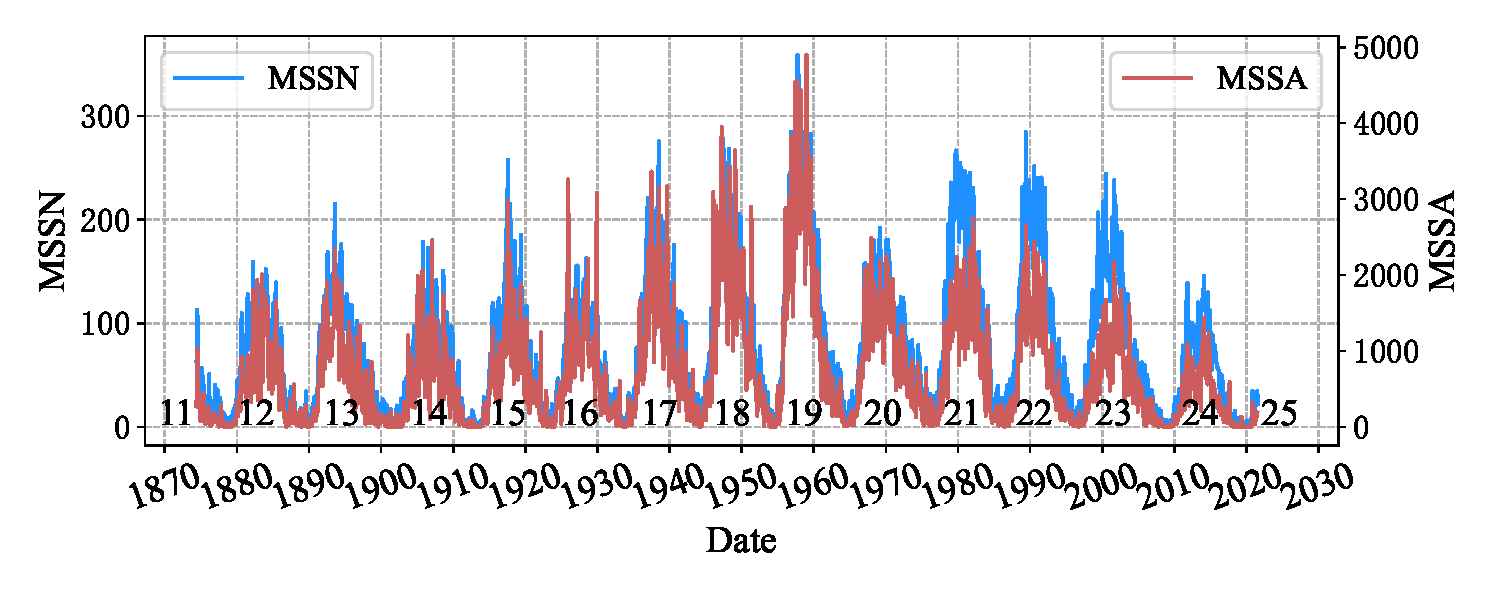
\includegraphics[width=\textwidth]{Img/chap3_ss/ss_number_area.pdf}
  \vspace{-1.4cm}
  \bicaption[1874年至2021年期间月均太阳黑子数和面积]{1874年至2021年期间月均太阳黑子数和面积。}{Monthly mean sunspot numbers and monthly mean sunspot areas from 1874 to 2021.}
  \label{fig:ss_number_area}
\end{figure}

为保持太阳黑子数和面积在时间上的一致性,将SSA数据集中的太阳黑子面积按月均,得到月均太阳黑子面积(Monthly Mean Sunspot Areas,简称MSSA)数据集。将MSSN和MSSA两种时间序列数据集绘制在同一张图中,可显示太阳黑子数和太阳黑子面积之间的动态变化关系。图\ref{fig:ss_number_area}截取了MSSA在1874年至2021年的数据集,纵轴按照不同尺度标准绘制太阳黑子数和太阳黑子面积的变化趋势。在重叠的时间范围内,太阳黑子数和面积在太阳活动强度和发生时间上存在高度的关联性。

\subsection{方法描述}\label{subsec:ss_method}

本节围绕预处理方法和机器学习模型展开。为了更精准地捕获太阳黑子变化趋势,本章使用了近几百年来观测到的太阳黑子数量/面积,使用不同种类的神经网络,试图从历史观测数据中提取关键信息,预测太阳黑子的动态变化特征。太阳黑子强度可以从长期历史记录中得到,依赖的历史时间长度从几个月到几个太阳周不等。将历史观测数据集转化为监督学习时间序列数据集。太阳黑子变化趋势可以被近似表达为:
\begin{equation}\adddotsbeforeeqnnum
  \label{eq:ss_sunspot_equation}
  S(t+\Delta,t+2\Delta,\ldots,t+f\Delta)=F[S(t,t-\Delta,\ldots,t-(k-1)\Delta)].
\end{equation}
其中,$\Delta$代表样本的采样间隔(1个月),$S(t+\Delta,t+2\Delta,\ldots,t+f\Delta)$代表未来$f$个月的太阳黑子强度,$S(t,t-\Delta,\ldots,t-(k-1)\Delta)$代表历史$k$个月的太阳黑子强度。

通过第\ref{sec:ml_slide}节的滑动窗口法,可以将原始太阳黑子数量数据集转换为监督学习数据集。紧接将数据集分割为训练集和测试集,分割比例为0.8:0.2。在训练集和测试集被使用之前,需要对两者分别进行归一化处理(第\ref{sec:ml_scaler}节)。MSSA数据集也进行了同样的操作。式\ref{eq:ss_sunspot_equation}明确指出,模型的输入是历史记录的太阳黑子数量/面积,输出为未来的太阳黑子数量/面积。

\section{试验结果与分析}\label{sec:ss_result}

太阳黑子时间序列呈现出复杂的非线性、非平稳型和非高斯型分布的特征。第\ref{sec:ml_cnn}节和第\ref{sec:ml_lstm}节提到,LSTM-RNN和1DCNN均适用于时间序列数据,而且原始记录持续了几百年,因此这里选择了LSTM-RNN和1DCNN。考虑到LSTM神经元、卷积运行在处理时间序列数据方面存在不同的优势,综合这两种优势,可以组成LSTM-1DCNN。

太阳黑子数据集记录的时间相对较长。MSSN数据集跨越了$\sim$273年,MSSA数据集跨越了$\sim$147年。引言\ref{sec:ss_intro}提到,太阳黑子变化存在周期性,平均为$\sim$11年。这里考虑输入时间窗口为72、132、264,评估不同输入时间窗口对模型的影响。每个输入响应可表示如下:
\begin{equation}\adddotsbeforeeqnnum
  \label{eq:ss_input}
  \begin{split}
    I_{-k}=[S(t),S(t-1),\ldots,S(t-k+1)].
  \end{split}
\end{equation}
其中,$k=72,132,264$。

本研究重点关注未来一个太阳周内的太阳黑子强度。为了预测第25太阳周的峰值,可以将输出时间窗口设置为72。将未来72个月太阳黑子最大值定义为第25太阳周的峰值。每个输出响应可以表示如下:
\begin{equation}\adddotsbeforeeqnnum
  \label{eq:ss_output}
  O_{+f}=[S(t+1),S(t+2),\ldots,S(t+f)].
\end{equation}
其中,$f=1,72$。

这里简要介绍不同模型的超参数配置。所有模型的输入节点数由输入时间窗口$k$决定,输出节点数由输出时间窗口$f$决定。以下是本章所有神经网络通用的超参数:训练经过1000回合;网络每层均使用线性整流函数(Rectified Linear Unit,简称ReLU)激活函数;批量训练的数据量设为132;Adam方法作为优化器;学习率初始值设为$10^{-3}$,同时训练次数每增加10次,学习率会减小$1-10^{-6}$倍;所有试验均使用“早停”策略。

\subsection{预测未来1个月太阳黑子强度}\label{sec:ss_result_1}

本节采用了三层LSTM-RNN、两层1DCNN和三层LSTM-1DCNN。因各种网络独特的性质,在设置以下超参数时会有所差异。针对LSTM-RNN,隐藏层含LSTM神经元,隐藏层的节点数分别设为64和32,最后一层为全连接层。针对1DCNN,隐藏层为一维卷积层,过滤器个数、过滤器大小、步长分别为32、3、2;卷积层后连接了最大池化层,池化大小为2,步长为1;最后一层为全连接层。针对LSTM-1DCNN,第一层含有LSTM神经元,神经元个数分别为64;第二层为一维卷积层,过滤器个数、过滤器大小、步长分别为16、3、1;最后一层为全连接层。 

\begin{table}[!htbp]
  \centering
  \bicaption[不同模型和输入时间窗口下预测未来1个月太阳黑子数的拟合指标效果]{不同模型和输入时间窗口下预测未来1个月太阳黑子数的拟合指标效果}{The indicators for predicting the next monthly sunspot numbers by different models with different input windows.}
  \label{tab:ss_number_out_1}
  \footnotesize
  \renewcommand{\arraystretch}{1}
  \begin{tabular}{ccccc}
    \toprule
    \multirow{2}{*}{模型} & \multirow{2}{*}{$I_{-k}$-[节点或过滤器数]-$O_{+f}$} & \multicolumn{2}{c}{测试集}\\
    \cmidrule(lr){3-4}
    \noalign{\smallskip}
    & & MSE & RMSE\\
    \midrule 
    LSTM-RNN & 72-[64-32]-1 & \textbf{0.0030} & \textbf{0.0548} \\
    LSTM-RNN & 132-[64-32]-1 & 0.0032 & 0.0569 \\
    LSTM-RNN & 264-[64-32]-1 & 0.0033 & 0.0578 \\
    \hline
    1DCNN & 72-[32]-1 & \textbf{0.0041} & \textbf{0.0640} \\
    1DCNN & 132-[32]-1 & 0.0042 & 0.0647 \\
    1DCNN & 264-[32]-1 & 0.0043 & 0.0658 \\
    \hline
    LSTM-1DCNN & 72-[64-32]-1 & \textbf{0.0029} & \textbf{0.0543} \\
    LSTM-1DCNN & 132-[64-32]-1 & 0.0032 & 0.0567 \\
    LSTM-1DCNN & 264-[64-32]-1 & 0.0032 & 0.0566 \\
    \bottomrule
  \end{tabular}
\end{table}

\begin{table}[!htbp]
  \centering
  \bicaption[最佳模型预测的太阳黑子强度]{最佳模型预测的太阳黑子强度。}{Prediction the sunspot amplitudes by the best models.}
  \label{tab:ss_out_1}
  \footnotesize
  \begin{tabular}{cccccc}
    \toprule
    日期 & 太阳黑子强度 & 输入时间窗口 & LSTM-RNN & 1DCNN & LSTM-1DCNN  \\
    \midrule
    2021年9月 & 数量 & 72个月 & 38.87 & 31.66 & \textbf{40.97} \\
    2021年8月 & 面积 & 72/132个月 & 274.14 & 359.78 & \textbf{288.61} \\
    \bottomrule
  \end{tabular}
\end{table}

讨论输出时间窗口为1个月时太阳黑子数。表\ref{tab:ss_number_out_1}展示了基于不同模型(LSTM-RNN、1DCNN和LSTM-1DCNN)、不同输入时间窗口(72、132、264)预测未来1个月太阳黑子数的拟合指标效果。表\ref{tab:ss_out_1}第一行展示了预测2021年9月太阳黑子数。就网络性能而言,LSTM-1DCNN性能略优于LSTM-RNN和1DCNN。就输入时间窗口而言,历史72个月的太阳黑子数作为时间窗口所得到的模型是最优的。当输入时间窗口为72个月时,LSTM-RNN的拟合指标较小(MSE=$0.0030$和RMSE=$0.0548$),预测2021年9月的太阳黑子数为$38.87$;1DCNN的拟合指标较小(MSE=$0.0041$和RMSE=$0.0640$),预测2021年9月的太阳黑子数为$31.66$;LSTM-1DCNN的拟合指标较小(MSE=$0.0029$和RMSE=$0.0543$),预测2021年9月的太阳黑子数为$40.97$。

讨论输出时间窗口为1个月时太阳黑子面积。表\ref{tab:ss_area_out_1}展示了使用不同模型(LSTM-RNN、1DCNN和LSTM-1DCNN)、不同输入时间窗口(72、132、264)预测未来1个月太阳黑子面积的拟合指标效果。表\ref{tab:ss_out_1}第二行展示了预测2021年8月太阳黑子面积。就网络性能而言,LSTM-1DCNN的性能同样略优于LSTM-RNN和1DCNN。当输入时间窗口为72个月时,LSTM-RNN的拟合指标较小(MSE=$0.0020$和RMSE=$0.0446$),预测2021年8月太阳黑子面积为$291.30$;当输入时间窗口为132个月时,1DCNN的拟合指标较小(MSE=$0.0028$和RMSE=$0.0531$),预测2021年8月太阳黑子面积为$359.78$;当输入时间窗口为132个月时,LSTM-1DCNN的拟合指标较小(MSE=$0.0021$和RMSE=$0.0453$),预测2021年8月太阳黑子面积为$288.61$。

\begin{table}[!htbp]
  \centering
  \bicaption[不同模型和输入时间窗口下预测未来1个月太阳黑子面积的拟合指标效果]{不同模型和输入时间窗口下预测未来1个月太阳黑子面积的拟合指标效果。}{The indicators for predicting the next monthly sunspot areas by different models with different input windows.}
  \label{tab:ss_area_out_1}
  \footnotesize
  \renewcommand{\arraystretch}{1}
  \begin{tabular}{ccccc}
    \toprule
    \multirow{2}{*}{模型} & \multirow{2}{*}{$I_{-k}$-[节点或过滤器数]-$O_{+f}$} & \multicolumn{2}{c}{测试集}\\
    \cmidrule(lr){3-4}
    \noalign{\smallskip}
    & & MSE & RMSE\\
    \midrule 
    LSTM & 72-[64-32]-1 & \textbf{0.0021} & \textbf{0.0454} \\
    LSTM & 132-[64-32]-1 & 0.0023 & 0.0479 \\
    LSTM & 264-[64-32]-1 & 0.0024 & 0.0492 \\
    \hline
    1DCNN & 72-[32]-1 & 0.0035 & 0.0588 \\
    1DCNN & 132-[32]-1 & \textbf{0.0028} & \textbf{0.0531} \\
    1DCNN & 264-[32]-1 & 0.0030 & 0.0551 \\
    \hline
    LSTM-1DCNN & 72-[64-32]-1 & 0.0021 & 0.0454 \\
    LSTM-1DCNN & 132-[64-32]-1 & \textbf{0.0021} & \textbf{0.0453} \\
    LSTM-1DCNN & 264-[64-32]-1 & 0.0023 & 0.0479 \\
    \bottomrule
\end{tabular}
\end{table}

\begin{figure}[!htbp]
  \centering
  \begin{subfigure}[b]{1.0\textwidth}
    \caption{LSTM-RNN} 
    \vspace{-0.35cm}
    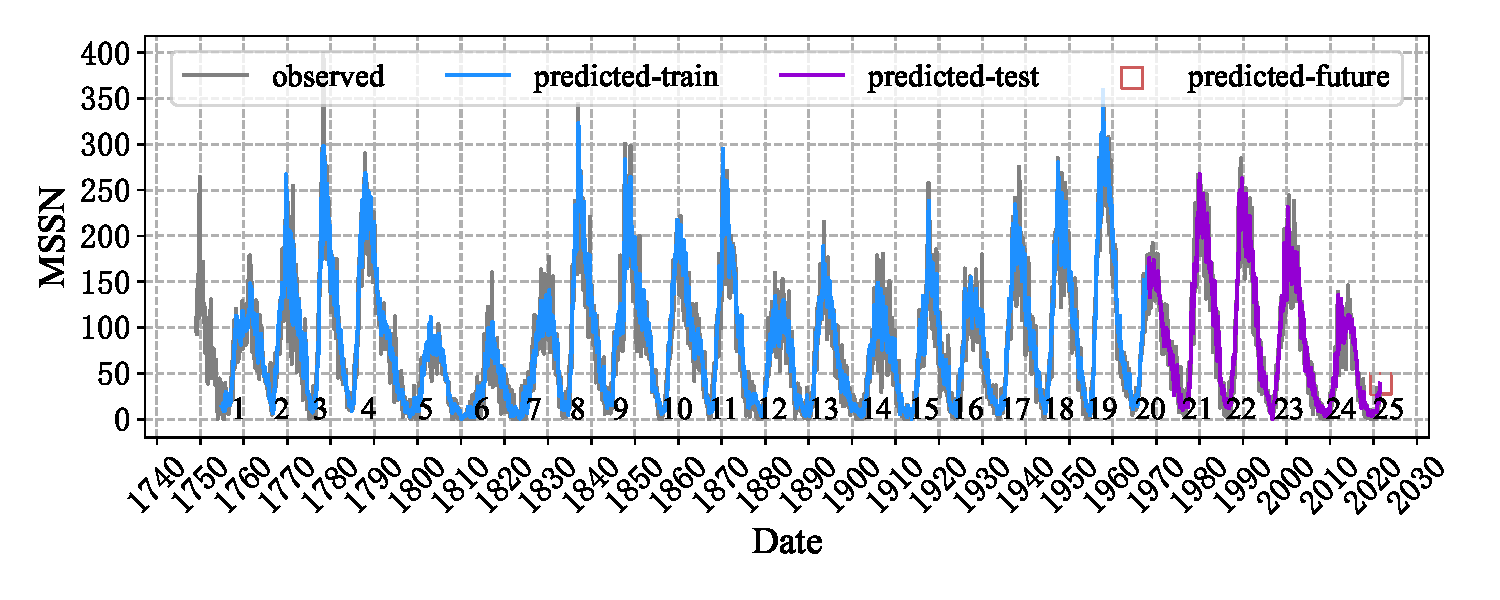
\includegraphics[width=\textwidth]{Img/chap3_ss/ssn_series_in_72_out_1_layer_3_layersize_64_lstm.pdf}
    \label{fig:ssn_series_in_72_out_1_lstm}
  \end{subfigure}    \\
  \vspace{-1cm}
  \begin{subfigure}[b]{1.0\textwidth}
    \caption{1DCNN}
    \vspace{-0.35cm}
    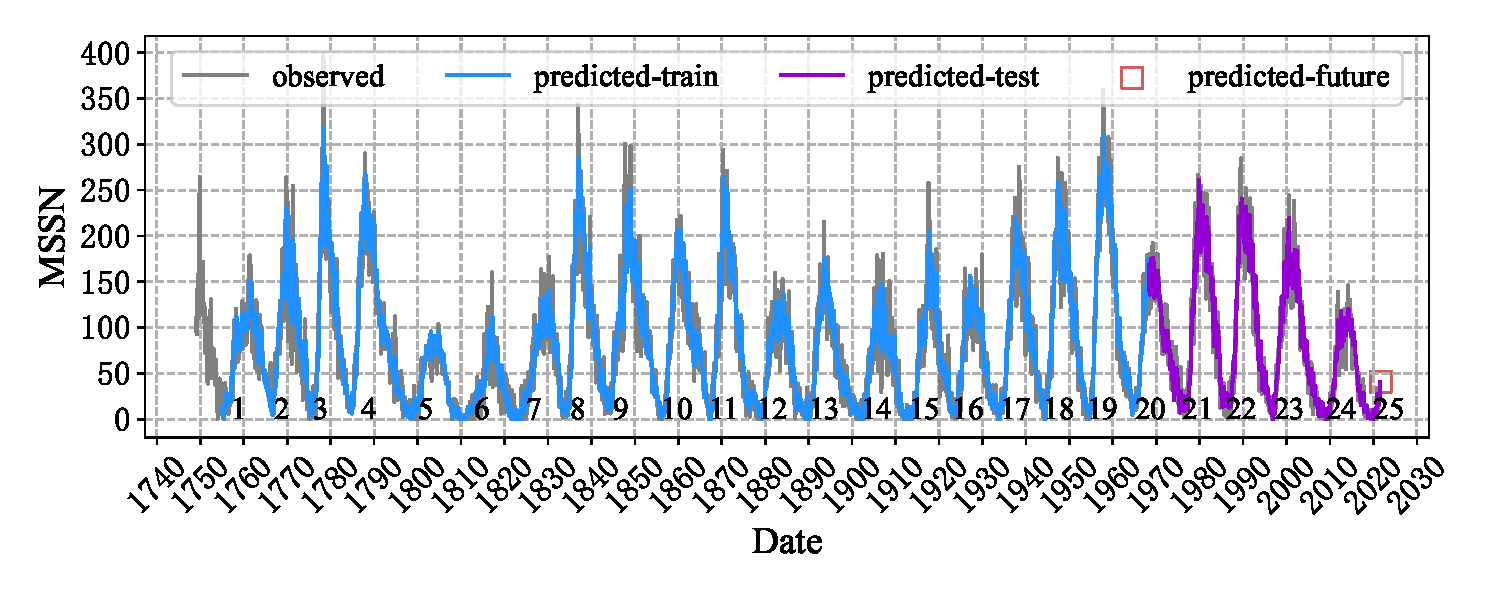
\includegraphics[width=\textwidth]{Img/chap3_ss/ssn_series_in_72_out_1_layer_3_layersize_64_lstm_cnn.pdf}
    \label{fig:ssn_series_in_72_out_1_cnn}
  \end{subfigure} \\
  \vspace{-1cm}
  \begin{subfigure}[b]{1.0\textwidth}
    \caption{LSTM-1DCNN}
    \vspace{-0.35cm}
    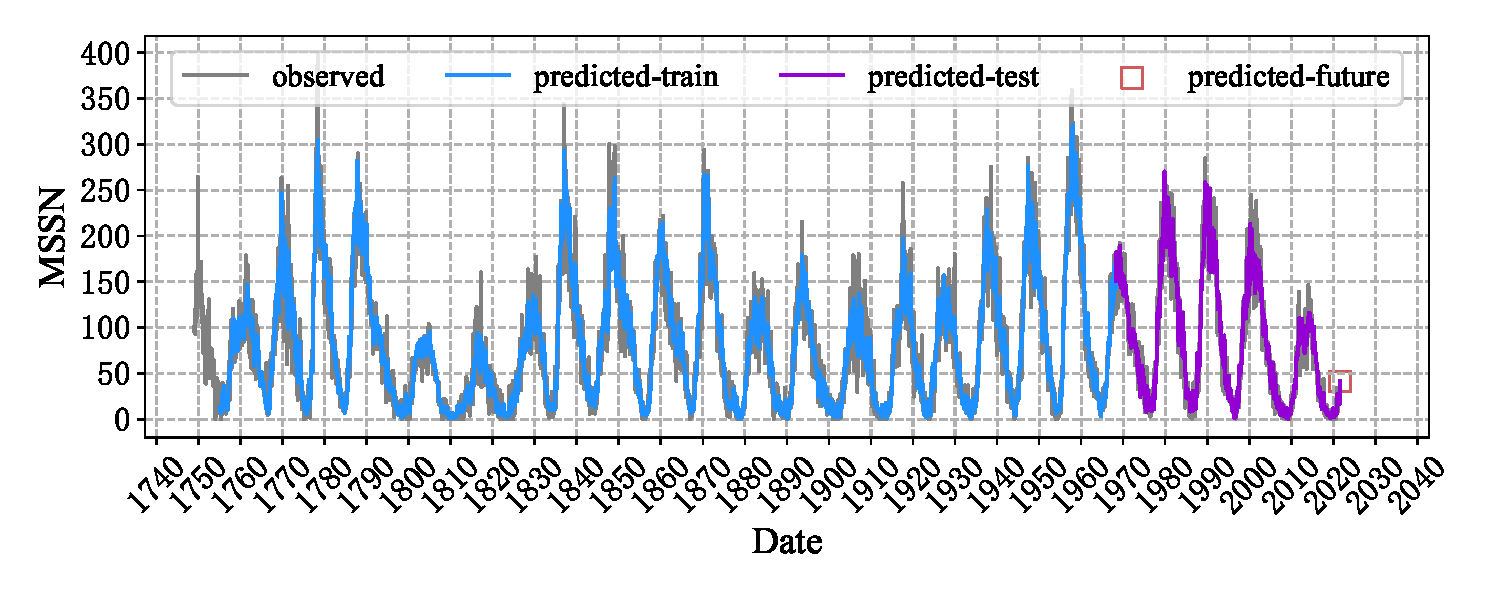
\includegraphics[width=\textwidth]{Img/chap3_ss/ssn_series_in_72_out_1_lstm_cnn.pdf}
    \label{fig:ssn_series_in_72_out_1_lstm_cnn}
    \end{subfigure}
  \vspace{-2cm}
  \bicaption[最佳模型预测未来1个月的太阳黑子数]{最佳模型预测未来1个月的太阳黑子数。}{Predicting the next monthly sunspot numbers by the best models.}
  \label{fig:ssn_series_in_72_out_1}
\end{figure}

\begin{figure}[!htbp]
  \centering
  \begin{subfigure}[b]{1.0\textwidth}
    \caption{LSTM-RNN} 
    \vspace{-0.35cm}
    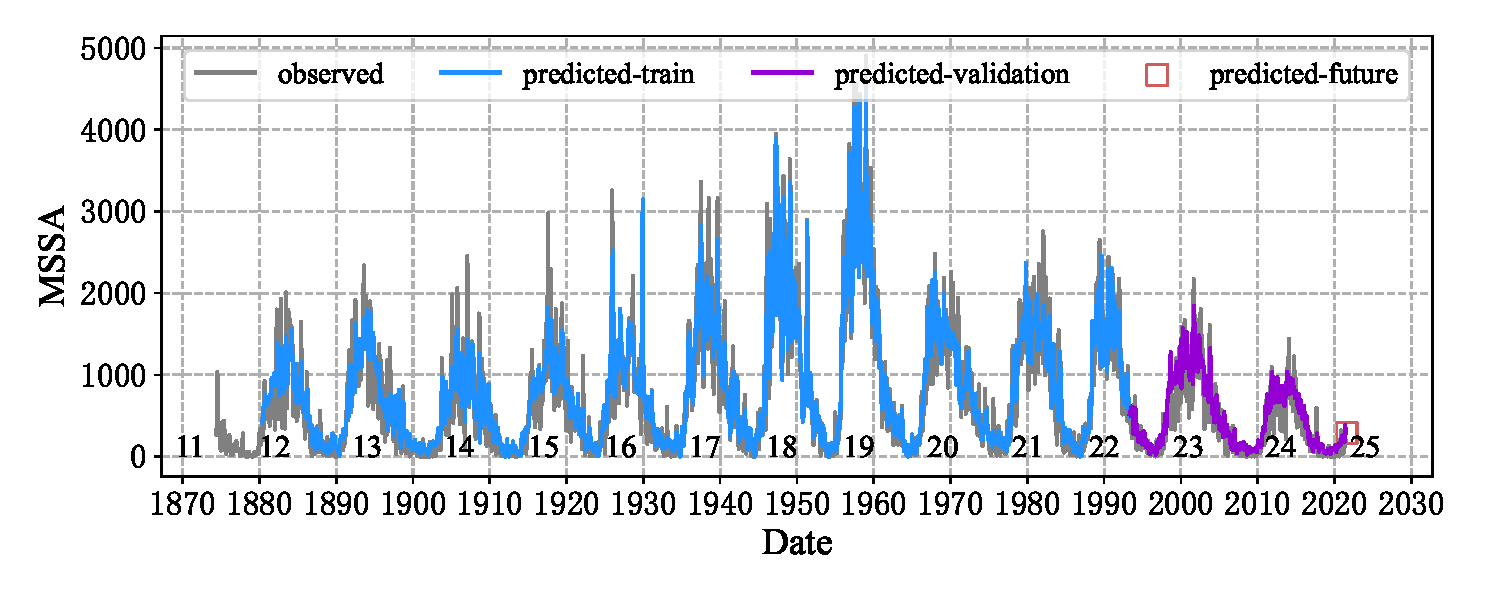
\includegraphics[width=\textwidth]{Img/chap3_ss/ssa_series_in_72_out_1_layer_3_layersize_64_lstm.pdf}
    \label{fig:ssa_series_in_132_out_1_lstm}
  \end{subfigure}    \\
  \vspace{-1cm}
  \begin{subfigure}[b]{1.0\textwidth}
    \caption{1DCNN}
    \vspace{-0.35cm}
    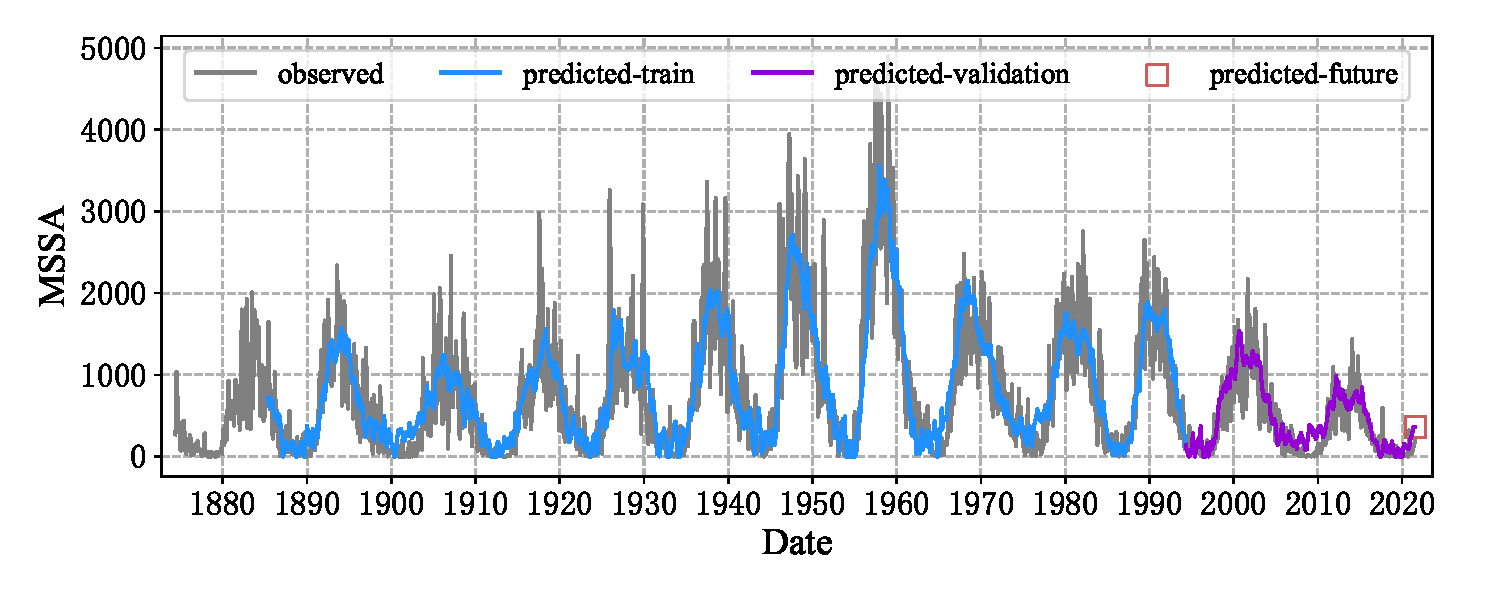
\includegraphics[width=\textwidth]{Img/chap3_ss/ssa_series_in_132_out_1_cnn.pdf}
    \label{fig:ssa_series_in_132_out_1_cnn}
  \end{subfigure} \\
  \vspace{-1cm}
  \begin{subfigure}[b]{1.0\textwidth}
    \caption{LSTM-1DCNN}
    \vspace{-0.35cm}
    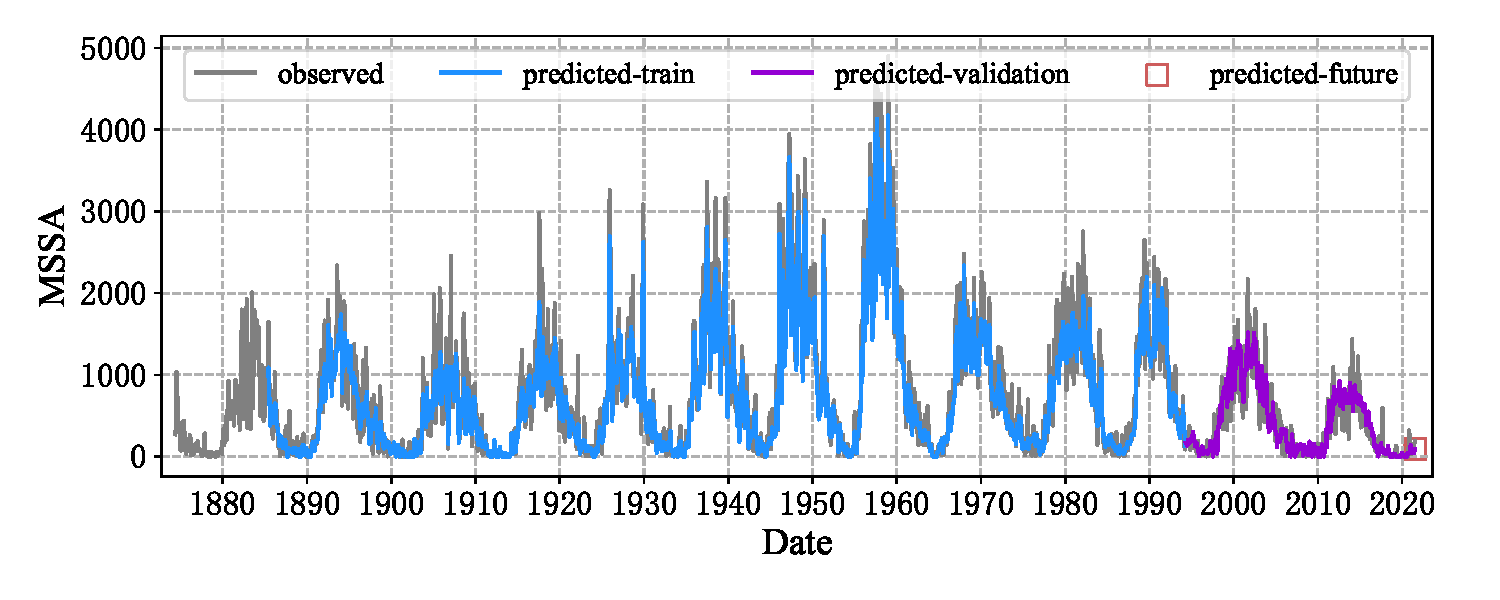
\includegraphics[width=\textwidth]{Img/chap3_ss/ssa_series_in_132_out_1_lstm_cnn.pdf}
    \label{fig:ssa_series_in_132_out_1_lstm_cnn}
    \end{subfigure}
  \vspace{-2cm}
  \bicaption[最佳模型预测未来1个月的太阳黑子面积]{最佳模型预测未来1个月的太阳黑子面积。}{Predicting the next monthly sunspot areas by the best models.}
  \label{fig:ssa_series_in_132_out_1}
\end{figure}

图\ref{fig:ssn_series_in_72_out_1}绘制了输入时间窗口为72的最佳模型预测未来1个月的太阳黑子数量,图\ref{fig:ssa_series_in_132_out_1}绘制了输入时间窗口为132的最佳模型预测未来1个月的太阳黑子面积。从图\ref{fig:ssn_series_in_72_out_1}和图\ref{fig:ssa_series_in_132_out_1}可以看出,对于预测值和测试集,LSTM-1DCNN具备良好的拟合能力。所有的结果均显示,预测的峰值比观测值略低,预测的谷值比观测值略高,这是因为太阳黑子强度较低或者较高时样本量偏少,模型难以准确学习到这些特征。

\subsection{预测未来72个月太阳黑子强度}\label{sec:ss_result_72}

\begin{table}[!htbp]
  \centering
  \bicaption[不同输入时间窗口和层数下LSTM-1DCNN预测未来72个月太阳黑子数的拟合指标效果]{不同输入时间窗口和层数下LSTM-1DCNN预测未来72个月太阳黑子数的拟合指标效果。}{The indicators for predicting the next 72 monthly sunspot numbers by LSTM-1DCNN with different input windows and layers.}
  \label{tab:ss_number_out_72}
  \footnotesize
  \renewcommand{\arraystretch}{1}
  \begin{tabular}{clccc}
    \toprule
    \multirow{2}{*}{层数} & \multirow{2}{*}{$I_{-k}$-[节点或过滤器数]-$O_{+f}$} & \multicolumn{2}{c}{测试集}\\
    \cmidrule(lr){3-4}
    \noalign{\smallskip}
    & & MSE & RMSE\\
    \midrule 
    3 & 72-[32(LSTM)-16(Conv)]-72 & 0.0189 & 0.1373 \\ 
      & 72-[64(LSTM)-32(Conv)]-72 & 0.0165 & 0.1283 \\
      & 72-[128(LSTM)-64(Conv)]-72 & 0.0140 & 0.1182 \\
      & 132-[32(LSTM)-16(Conv)]-72 & 0.0195 & 0.1397 \\
      & 132-[64(LSTM)-32(Conv)]-72 & 0.0124 & 0.1115 \\
      & 132-[128(LSTM)-64(Conv)]-72 & 0.0133 & 0.1151 \\
      & 264-[32(LSTM)-16(Conv)]-72 & 0.0155 & 0.1245 \\
      & 264-[64(LSTM)-32(Conv)]-72 & 0.0122 & 0.1103 \\
      & 264-[128(LSTM)-64(Conv)]-72 & \textbf{0.0085} & \textbf{0.0920} \\
    \hline
    4 & 72-[64(LSTM)-32(LSTM)-16(Conv)]-72 & 0.0179 & 0.1339 \\
      & 72-[128(LSTM)-64(LSTM)-32(Conv)]-72 & 0.0135 & 0.1162  \\
      & 72-[256(LSTM)-128(LSTM)-64(Conv)]-72 & 0.0146 & 0.1206 \\
      & 132-[64(LSTM)-32(LSTM)-16(Conv)]-72 & 0.0170 & 0.1305 \\
      & 132-[128(LSTM)-64(LSTM)-32(Conv)]-72 & 0.0132 & 0.1148 \\
      & 132-[256(LSTM)-128(LSTM)-64(Conv)]-72 & 0.0149 & 0.1220 \\
      & 264-[64(LSTM)-32(LSTM)-16(Conv)]-72 & 0.0089 & 0.0944 \\
      & 264-[128(LSTM)-64(LSTM)-32(Conv)]-72 & \textbf{0.0071} & \textbf{0.0841} \\
      & 264-[256(LSTM)-128(LSTM)-64(Conv)]-72 & 0.0093 & 0.0965 \\
    \hline
    5 & 72-[128(LSTM)-64(LSTM)-32(LSTM)-21(Conv)]-72 & 0.0173 & 0.1315 \\
      & 72-[256(LSTM)-128(LSTM)-64(LSTM)-42(Conv)]-72 & 0.0134 & 0.1157 \\
      & 72-[512(LSTM)-256(LSTM)-128(LSTM)-85(Conv)]-72 & 0.0158 & 0.1258 \\
      & 132-[128(LSTM)-64(LSTM)-32(LSTM)-21(Conv)]-72 & 0.0150 & 0.01226 \\
      & 132-[256(LSTM)-128(LSTM)-64(LSTM)-42(Conv)]-72 & 0.0163 & 0.1276 \\
      & 132-[512(LSTM)-256(LSTM)-128(LSTM)-85(Conv)]-72 & 0.0161 &  0.1268\\
      & 264-[128(LSTM)-64(LSTM)-32(LSTM)-21(Conv)]-72 & 0.0087 & 0.0935 \\
      & 264-[256(LSTM)-128(LSTM)-64(LSTM)-42(Conv)]-72 & \textbf{0.0072} & \textbf{0.0849} \\
      & 264-[512(LSTM)-256(LSTM)-128(LSTM)-85(Conv)]-72 & 0.0074 & 0.0859 \\
    \bottomrule
  \end{tabular}
\end{table}

第\ref{sec:ss_result_1}节预测未来1个月太阳黑子数量/面积时,得出LSTM-1DCNN性能略优于LSTM-RNN和1DCNN。同时考虑到LSTM-1DCNN结合了LSTM-RNN和1DCNN两者的优点,以下试验不再考虑LSTM-RNN和1DCNN两种模型。本节讨论输出时间窗口为72个月的太阳黑子强度。表\ref{tab:ss_number_out_72}展示了不同架构的LSTM-1DCNN模型在不同输入时间窗口(72、132、264)下预测未来72个月太阳黑子数的拟合指标效果。与表\ref{tab:ss_number_out_1}相比,表\ref{tab:ss_number_out_72}中MSE值和RMSE值出现了一定程度的增加。也就是说,随着输出时间窗口的增加,模型性能呈现下降趋势。在相同的输入时间窗口下,隐藏层层数和节点数越多,模型性能先上升后下降。就输入时间窗口而言,历史264个月的太阳黑子数作为输入时间窗口所得到的模型是最优的。

\begin{table}[!htbp]
\centering
\bicaption[最佳模型预测未来72个月太阳黑子强度的最大值]{最佳模型预测未来72个月太阳黑子强度的最大值。}{Prediction the sunspot maximum amplitudes by the best models.}
\label{tab:ss_out_72}
\footnotesize
\begin{tabular}{cccccccc}
    \toprule
    &  & \multicolumn{2}{c}{3层} & \multicolumn{2}{c}{4层} & \multicolumn{2}{c}{5层}\\
    \cmidrule(lr){3-4} \cmidrule(lr){5-6} \cmidrule(lr){7-8}
    \noalign{\smallskip}
     & 输入时间窗口 & 最大值 & 发生时间 & 最大值 & 发生时间 & 最大值 & 发生时间 \\
    \midrule
    数量 & 264 & 151.55 & 2023年9月 & 174.71 & 2025年1月 & \textbf{132.86} & \textbf{2024年12月} \\
    面积 & 132/264/72 & 1016.32 & 2024年8月 & \textbf{1469.01} & \textbf{2025年3月} & 1397.77 & 2024年4月 \\
    \bottomrule
  \end{tabular}
\end{table}

表\ref{tab:ss_out_72}第一行展示了最佳模型预测未来72个月最大的太阳黑子数和出现时间。当输入时间窗口为264个月时,3层的LSTM-1DCNN的拟合指标较小(MSE=$0.0085$和RMSE=$0.0920$),预测未来72个月的太阳黑子数的最大值为$151.55$,出现在2023年9月;4层的LSTM-1DCNN的拟合指标较小(MSE=$0.0082$和RMSE=$0.0905$),预测未来72个月的太阳黑子数最大值为$174.71$,出现在2025年1月;5层的LSTM-1DCNN的拟合指标较小(MSE=$0.0072$和RMSE=$0.0849$),预测未来72个月的太阳黑子数的最大值为$132.86$,出现在2024年12月。对黑子数而言,第23太阳周最大MSSN出现在2001年9月,其值为238.2;第24太阳周最大MSSN出现在2014年2月,其值为146.1。研究结果显示,第25太阳周的峰值跟第24太阳周基本持平。 

\begin{figure}[!htbp]
  \centering
  \begin{subfigure}[b]{1.0\textwidth}
    \caption{264-[128(LSTM)-64(Conv)]-72} 
    \vspace{-0.35cm}
    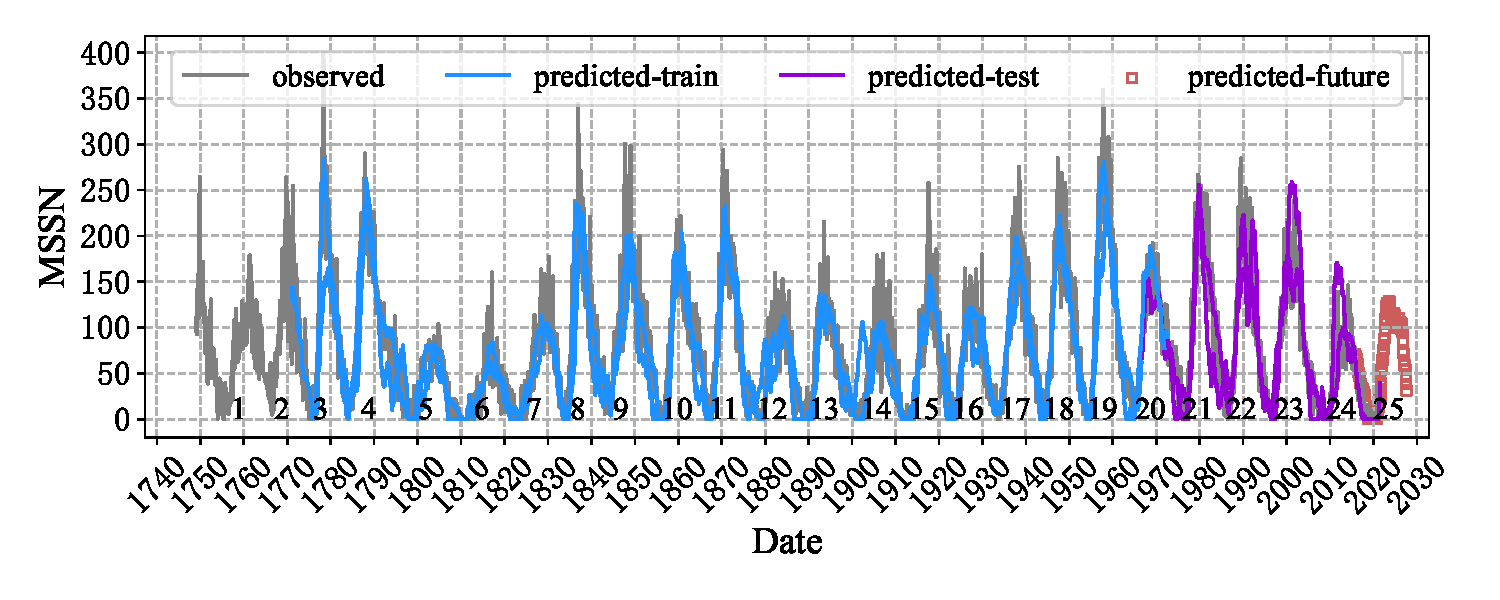
\includegraphics[width=\textwidth]{Img/chap3_ss/ssn_series_in_264_out_72_layer_3_layersize_128_lstm_cnn.pdf}
    \label{fig:ssn_series_in_264_out_72_layer_3_layersize_128_lstm_cnn}
  \end{subfigure}    \\
  \vspace{-1cm}
  \begin{subfigure}[b]{1.0\textwidth}
    \caption{264-[128(LSTM)-64(LSTM)-32(Conv)]-72}
    \vspace{-0.35cm}
    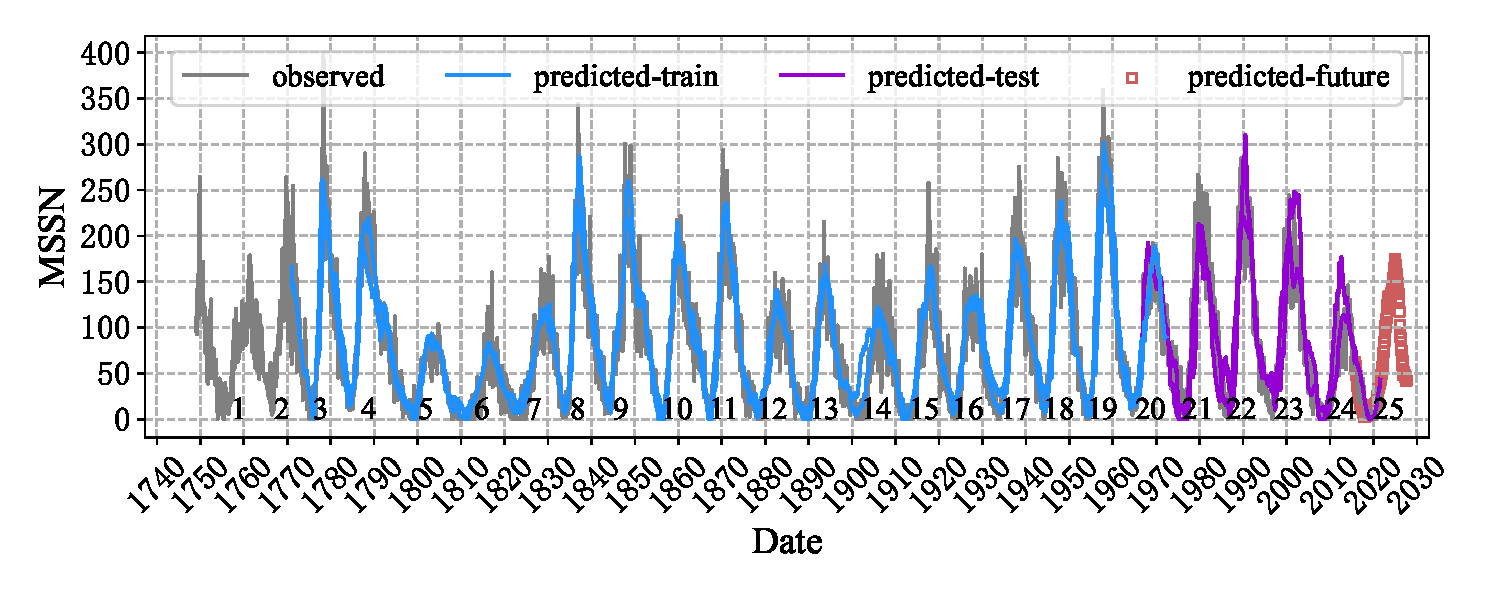
\includegraphics[width=\textwidth]{Img/chap3_ss/ssn_series_in_264_out_72_layer_4_layersize_128_lstm_cnn.pdf}
    \label{fig:ssn_series_in_264_out_72_layer_4_layersize_128_lstm_cnn}
  \end{subfigure} \\
  \vspace{-1cm}
  \begin{subfigure}[b]{1.0\textwidth}
    \caption{264-[256(LSTM)-128(LSTM)-64(LSTM)-42(Conv)]-72}
    \vspace{-0.35cm}
    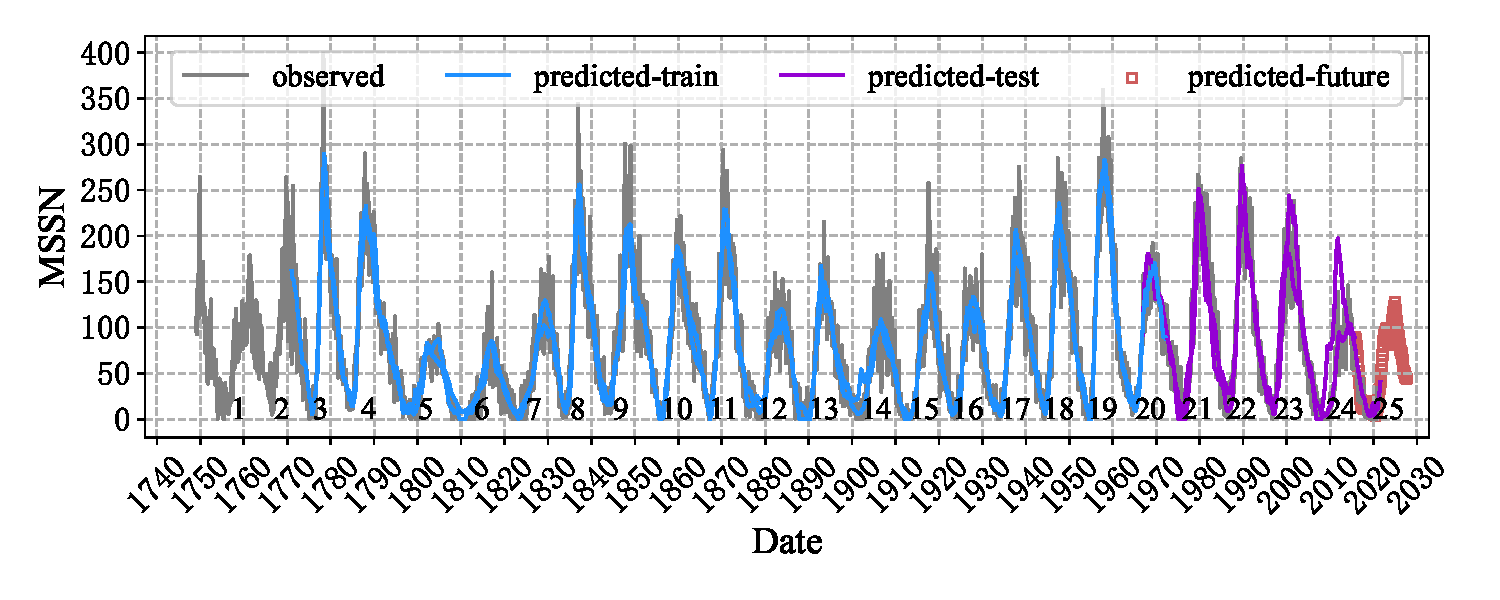
\includegraphics[width=\textwidth]{Img/chap3_ss/ssn_series_in_264_out_72_layer_5_layersize_256_lstm_cnn.pdf}
    \label{fig:ssn_series_in_264_out_72_layer_5_layersize_256_lstm_cnn}
    \end{subfigure}
  \vspace{-2cm}
  \bicaption[最佳模型预测未来72个月的太阳黑子数]{最佳模型预测未来72个月的太阳黑子数。}{Predicting the next 74 monthly sunspot numbers by the best models.}
  \label{fig:ssn_series_in_264_out_72_lstm_cnn}
\end{figure}

图\ref{fig:ssn_series_in_264_out_72_lstm_cnn}绘制了不同结构的LSTM-1DCNN的最佳模型预测未来72个月的太阳黑子数。为了更清晰地展示结果,图\ref{fig:ssn_series_in_264_out_72_lstm_cnn}在绘制训练集和测试集的结果时,只绘制了每个输入样本的第一个和最后一个预测值。图\ref{fig:ssn_series_in_264_out_72_lstm_cnn}显示,未来第72个月太阳黑子数的最大值与第24太阳周的峰值基本持平,而且在第25太阳周出现了双峰性质。相比于图\ref{fig:ssn_series_in_264_out_72_layer_4_layersize_128_lstm_cnn}和图\ref{fig:ssn_series_in_264_out_72_layer_5_layersize_256_lstm_cnn},图\ref{fig:ssn_series_in_264_out_72_layer_3_layersize_128_lstm_cnn}中的第一个峰值比第二个大,导致预测的峰值出现的时间提前。

\begin{table}[!htbp]
  \centering
  \bicaption[不同输入时间窗口和层数的LSTM-1DCNN预测未来72个月太阳黑子面积的拟合指标效果]{不同输入时间窗口和层数的LSTM-1DCNN预测未来72个月太阳黑子面积的拟合指标效果。}{The indicators for predicting the next 72 monthly sunspot areas by LSTM-1DCNN with different input windows and layers.}
  \label{tab:ss_area_out_72}
  \footnotesize
  \renewcommand{\arraystretch}{1}
  \begin{tabular}{clccc}
    \toprule
    \multirow{2}{*}{模型} & \multirow{2}{*}{$I_{-k}$-[节点或过滤器数]-$O_{+f}$} & \multicolumn{2}{c}{测试集}\\
    \cmidrule(lr){3-4}
    \noalign{\smallskip}
    & & MSE & RMSE\\
    \midrule 
    3 & 72-[32(LSTM)-16(Conv)]-72 & 0.0105 & 0.1025 \\ 
      & 72-[64(LSTM)-32(Conv)]-72 & 0.0085 & 0.0923 \\
      & 72-[128(LSTM)-64(Conv)]-72 & 0.0097 & 0.0987 \\
      & 132-[32(LSTM)-16(Conv)]-72 & 0.0093 & 0.0965 \\
      & 132-[64(LSTM)-32(Conv)]-72 & 0.0091 & 0.0952 \\
      & 132-[128(LSTM)-64(Conv)]-72 & \textbf{0.0078} & \textbf{0.0884} \\
      & 264-[32(LSTM)-16(Conv)]-72 & 0.0091 & 0.0956 \\
      & 264-[64(LSTM)-32(Conv)]-72 & 0.0090 & 0.0950 \\
      & 264-[128(LSTM)-64(Conv)]-72 & 0.0084 & 0.0919 \\
    \hline
    4 & 72-[64(LSTM)-32(LSTM)-16(Conv)]-72 & 0.0107 & 0.1036 \\
      & 72-[128(LSTM)-64(LSTM)-32(Conv)]-72 & 0.0097 & 0.0986 \\
      & 72-[256(LSTM)-128(LSTM)-64(Conv)]-72 & 0.0099 & 0.0993 \\
      & 132-[64(LSTM)-32(LSTM)-16(Conv)]-72 & 0.0100 & 0.0998 \\
      & 132-[128(LSTM)-64(LSTM)-32(Conv)]-72 & 0.0091 & 0.0953 \\
      & 132-[256(LSTM)-128(LSTM)-64(Conv)]-72 & 0.0091 & 0.0953\\
      & 264-[64(LSTM)-32(LSTM)-16(Conv)]-72 & 0.0096 & 0.0978 \\
      & 264-[128(LSTM)-64(LSTM)-32(Conv)]-72 & 0.0075 & 0.0865 \\
      & 264-[256(LSTM)-128(LSTM)-64(Conv)]-72 & \textbf{0.0054} & \textbf{0.0733} \\
    \hline
    5 & 72-[128(LSTM)-64(LSTM)-32(LSTM)-21(Conv)]-72 & 0.0105 & 0.1023 \\
      & 72-[256(LSTM)-128(LSTM)-64(LSTM)-42(Conv)]-72 & 0.0071 & 0.0841 \\
      & 72-[512(LSTM)-256(LSTM)-128(LSTM)-85(Conv)]-72 & \textbf{0.0061} & \textbf{0.0781} \\
      & 132-[128(LSTM)-64(LSTM)-32(LSTM)-21(Conv)]-72 & 0.0089 & 0.0941 \\
      & 132-[256(LSTM)-128(LSTM)-64(LSTM)-42(Conv)]-72 & 0.0063 & 0.0791 \\
      & 132-[512(LSTM)-256(LSTM)-128(LSTM)-85(Conv)]-72 & 0.0067 & 0.0817 \\
      & 264-[128(LSTM)-64(LSTM)-32(LSTM)-21(Conv)]-72 & 0.0101 & 0.1006 \\
      & 264-[256(LSTM)-128(LSTM)-64(LSTM)-42(Conv)]-72 & 0.0075 & 0.0867 \\
      & 264-[512(LSTM)-256(LSTM)-128(LSTM)-85(Conv)]-72 & 0.0096 & 0.0980 \\
    \bottomrule
\end{tabular}
\end{table}

表\ref{tab:ss_out_72}第二行展示了预测的未来72个月最大的太阳黑子面积和出现时间。3层最佳的LSTM-1DCNN模型的输入时间窗口为132个月时,拟合指标为MSE=$0.0078$,RMSE=$0.0884$,预测未来72个月太阳黑子面积最大值为$1016.32$,出现在2024年8月;4层最佳的LSTM-1DCNN的拟合指标MSE=$0.0082$,RMSE=$0.0905$,预测未来72个月太阳黑子面积最大值为$1469.01$,出现在2025年3月;5层最佳的LSTM-1DCNN的拟合指标为MSE=$0.0072$,RMSE=$0.0849$,预测未来72个月太阳黑子面积最大值为$1397.77$,出现在2024年4月。对于太阳黑子面积,第23太阳周MSSA的峰值为2171.7,出现在2001年9月;第24太阳周MSSA的峰值为1439.82,出现在2014年2月。研究结果显示,第25太阳周的峰值跟第24太阳周基本持平。 

\begin{figure}[!htbp]
  \centering
  \begin{subfigure}[b]{1.0\textwidth}
    \caption{3层(132-[128(LSTM)-64(Conv)]-72)} 
    \vspace{-0.35cm}
    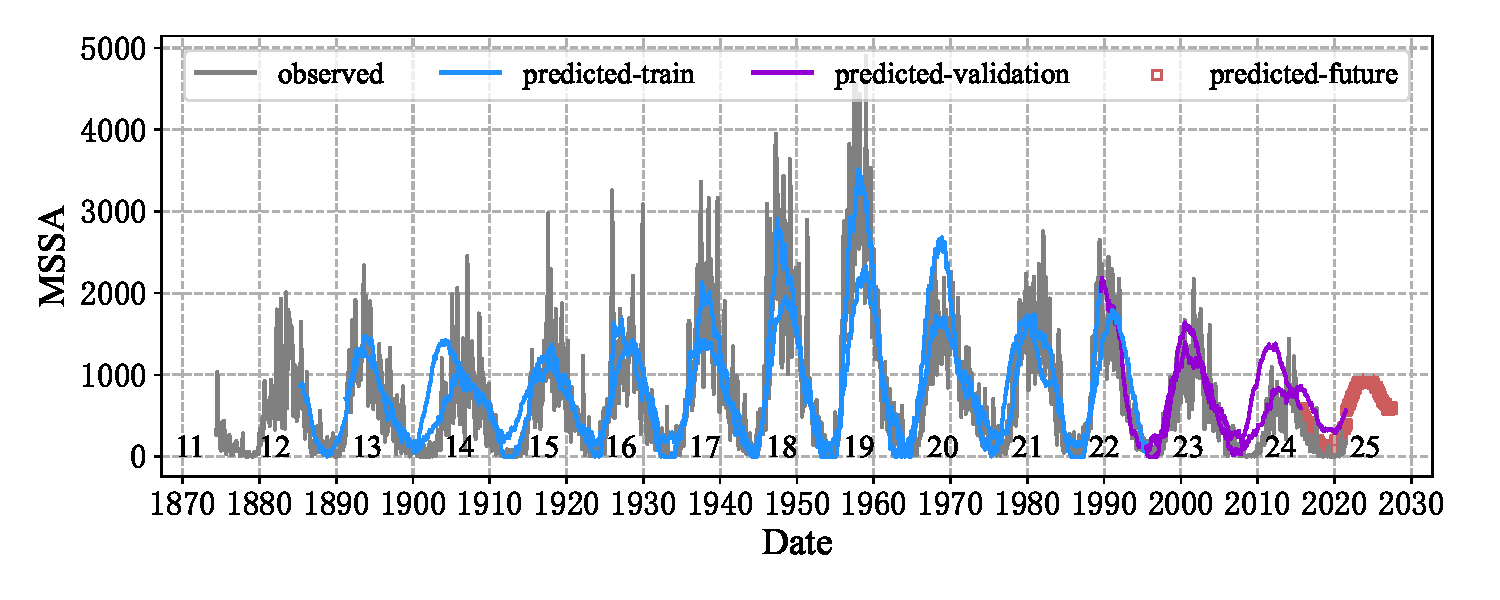
\includegraphics[width=\textwidth]{Img/chap3_ss/ssa_series_in_132_out_72_layer_3_layersize_128_lstm_cnn.pdf}
    \label{fig:ssa_series_in_132_out_72_layer_3_layersize_128_lstm_cnn}
  \end{subfigure}    \\
  \vspace{-1cm}
  \begin{subfigure}[b]{1.0\textwidth}
    \caption{4层(264-[256(LSTM)-128(LSTM)-64(Conv)]-72)}
    \vspace{-0.35cm}
    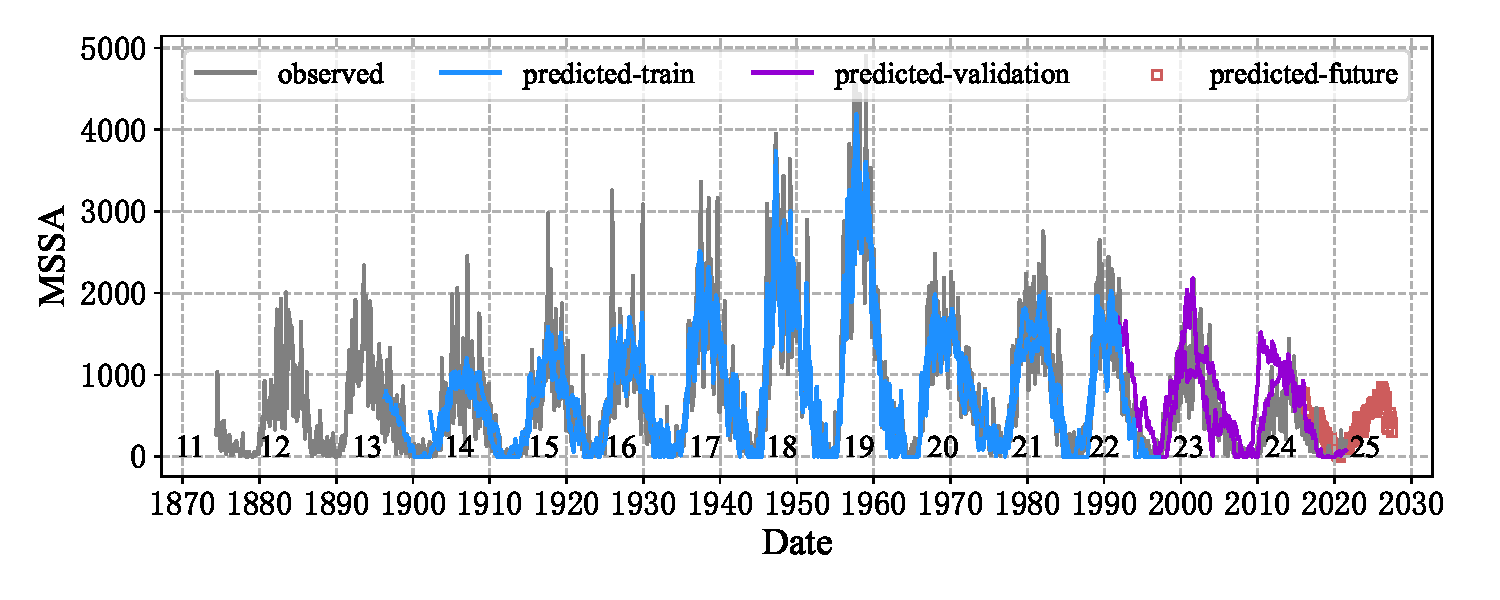
\includegraphics[width=\textwidth]{Img/chap3_ss/ssa_series_in_264_out_72_layer_4_layersize_256_lstm_cnn.pdf}
    \label{fig:ssa_series_in_264_out_72_layer_4_layersize_256_lstm_cnn}
  \end{subfigure} \\
  \vspace{-1cm}
  \begin{subfigure}[b]{1.0\textwidth}
    \caption{5层(72-[512(LSTM)-256(LSTM)-128(LSTM)-85(Conv)]-72)}
    \vspace{-0.35cm}
    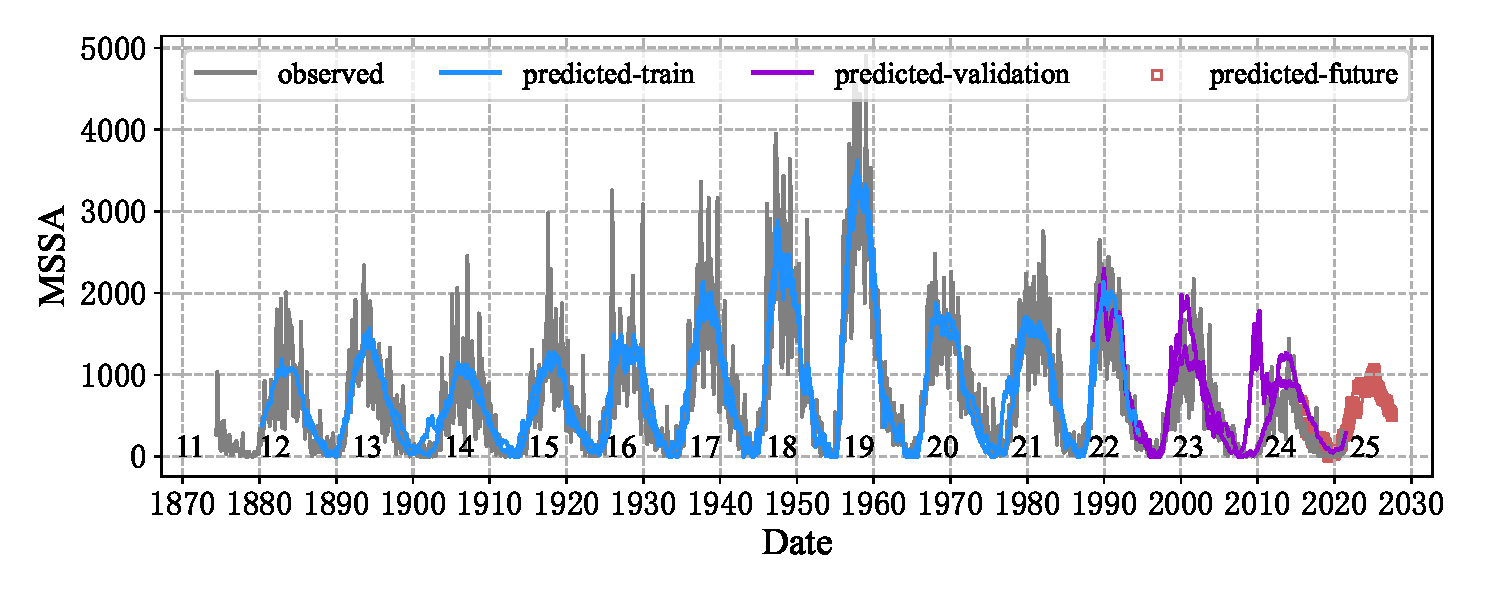
\includegraphics[width=\textwidth]{Img/chap3_ss/ssa_series_in_72_out_72_layer_5_layersize_512_lstm_cnn.pdf}
    \label{fig:ssa_series_in_72_out_72_layer_5_layersize_512_lstm_cnn}
    \end{subfigure}
  \vspace{-2cm}
  \bicaption[最佳模型预测未来72个月的太阳黑子面积]{最佳模型预测未来72个月的太阳黑子面积。}{Predicting the next 72 monthly sunspot areas by the best models.}
  \label{fig:ssa_series_out_72_lstm_cnn}
\end{figure}

为了更清晰地展示结果,在展示训练集和测试集的结果时,只绘制了每个输入样本的第一个和最后一个预测值。图\ref{fig:ssa_series_out_72_lstm_cnn}绘制了不同结构的LSTM-1DCNN的最佳模型预测未来72个月的太阳黑子面积。图\ref{fig:ssa_series_out_72_lstm_cnn}显示,未来第72个月超过了在第25太阳周峰值的到达时间。图\ref{fig:ssa_series_in_132_out_72_layer_3_layersize_128_lstm_cnn}和图\ref{fig:ssa_series_in_72_out_72_layer_5_layersize_512_lstm_cnn}均在第25太阳周均出现了双峰性质。

图\ref{fig:ssn_series_in_264_out_72_lstm_cnn}和图\ref{fig:ssa_series_out_72_lstm_cnn}分别绘制了不同层数下最佳模型预测太阳黑子数量和面积。从图\ref{fig:ssn_series_in_264_out_72_lstm_cnn}和图\ref{fig:ssa_series_out_72_lstm_cnn}可以看出,对于预测值和测试集,LSTM-1DCNN具备良好的拟合能力。所有的结果均显示,预测的峰值比观测值略低,预测的谷值比观测值略高,因为太阳黑子强度较低或较高的样本量偏少,模型难以准确学习到这些特征。

\subsection{与其他研究的比较}\label{sec:ss_result_compare}

\begin{table}[!htbp]
  \bicaption[不同研究给出的预测第25太阳周的太阳黑子强度相比于第24太阳周的强弱]{不同研究给出的预测第25太阳周的太阳黑子强度相比于第24太阳周的强弱}{The different studies for predicting sunspot amplitude of cycle 25 comparing with cycle 24.}
  \label{tab:ss_number_different_studies}
  \centering
  \footnotesize
  \begin{tabular}{llll}
    \toprule 
    方法 & 相比第24太阳周 & 峰值达到时间 & 参考文献  \\
    \midrule
    LSTM-1DCNN & 基本相等 & 2024年12月--2025年3月 & 本研究 \\
    
    
    
    
    光谱分量外推法 & 29\% 更强 & 2022年至2023年之间 & \citet{kane2007solar}\\
    光谱小波分解树 & 17\% 更强 & 2023年4月 & \citet{rigozo2011prediction} \\
    多维混合神经网络 & 基本相等 & 2025年1月(\pm 6个月)& \citet{okoh2018hybrid} \\
    线性回归 & 10\%更强 & 2023年9月 & \citet{dani2019prediction}\\
    前向传播神经网络 & 更弱 & 2022年至2023年左右 & \citet{covas2019neural} \\
    相似周期方法 & 30\% 更强 & 2024年10月& \citet{du2020solar} \\
    LSTM-RNN & 55\% 更强 & 2022年10月 & \citet{li2021predicting} \\
    \bottomrule
\end{tabular}
\end{table}

已有很多研究中采取不同的方法预测即将到来的第25太阳周的太阳黑子变化,得到结果并不统一。可能原因是太阳黑子具备极其复杂的易变性、数据集长度的差异、预处理的差异以及选择模型的差异等。表\ref{tab:ss_number_different_studies}列出部分关于第25太阳周的研究。例如,\citet{covas2019neural}使用具备时空特性的神经网络,预测第25太阳周可能是有史以来太阳黑子数最低的时期,预测峰值出现的时间为2022年至2023年。\citet{okoh2018hybrid}利用多维混合模型估计MSSN,得到第25太阳周的峰值为122.1(\pm 18.2),达到时间为2025年1月(\pm 6个月)。

\section{讨论与小结}\label{sec:ss_conclusion}

\citet{solanki2011analyzing}指出不同的关于长期预测太阳黑子变化研究得出的结论差异较大,这主要是因为太阳黑子变化具有非常复杂的非线性特征。MSSN和MSSA时间序列数据是非稳态的,数据中所包含的随机的分量使太阳黑子在长时间预测尺度上不太可靠。由于数据中含有非线性效应的随机波动,难以对未来几个周期进行准确预测\citep{charbonneau2010dynamo,petrovay2010solar}。\citet{charbonneau2010dynamo}认为,传统物理的物理模型没有建立在观测数据,难以反应真实情况。\citet{mendoza2011mid}指出,太阳黑子活动起源于一定范围内的周期过程,而不是随机或间歇性过程。

截至目前,太阳黑子预测最大的挑战是预测下一太阳周的最大振幅和持续时间\citep{petrovay2010solar}。\citet{gleissberg1939long}曾指出太阳黑子周期的波动不够规则,在获取响应的表达函数时相当困难。\citet{herrera2015reconstruction}假设太阳黑子每个周期存在一个固定的能量和给定频率(即太阳黑子活动周期在8年至14年之间),则太阳黑子估计模型的准确度会受到不确定原则的限制。因此,准确预测太阳黑子的任何参数(相位、振幅和周期)都十分困难。不仅未来太阳周期的特性难以预测,而且准确预知太阳黑子强度也几乎不可能。太阳黑子周期预测的问题可被视作一个概率问题。这也是太阳周期预测中经常会出现太阳黑子周期的预测概率。\citet{camporeale2019challenge}建议在空间天文研究中需要改变预测模式,从点预测到具有可靠不确定性的概率方法。太阳周期的振幅取决于其在震荡阶段的位置变化,理论上可以定性预测第25太阳周的最大振幅。然而,不同的物理模型和数值模型预测未来太阳周最大振幅时还存在较大差异。

本研究使用了LSTM-RNN、1DCNN以及LSTM-1DCNN预测未来太阳黑子变化,采用了MSSN和MSSA数据集,发现第25太阳周的最大太阳黑子数为132.86(发生在2024年12月),最大太阳黑子面积为1469.01(发生在2025年3月)。预测结果与\citet{covas2019neural}的研究结果不仅在黑子强度上类似,而且在发生时间上也相近。

同时研究还发现,模型性能会随着输出时间窗口的增加而略微下降,随着层数和节点数的增加而略微上升。如果要提供非常准确的预报,可以将输出时长设置为1年,每隔一段时间更新模型,重新预测下一年的太阳黑子变化。这也是本方法在太阳黑子预测上的局限性。输入时间窗口和输出时间窗口直接决定了模型的构建,而且输出时间窗口对预测结果有非常大的影响,这使得合适的输出序列长度成为良好模型构建的一项前提条件。
